
%\usepackage{graphicx}

%%%%%%%%%%%%%%%%%%%%%%%%%%%
%\usepackage{srcltx}
%%%%%%%%%%%%%%%%%%%%%%%%%%%%%%

\begin{titlepage}

\large \thispagestyle{empty} \phantom{.}\vspace{2mm} \large
\thispagestyle{empty}

\begin{center}
%МИНИСТЕРСТВО НАУКИ И ОБРАЗОВАНИЯ\\
%РОССИЙСКОЙ ФЕДЕРАЦИИ\\
%\bigskip
МОСКОВСКИЙ ГОСУДАРСТВЕННЫЙ УНИВЕРСИТЕТ\\
ИМ. М.В.ЛОМОНОСОВА\\
\noindent\

\vspace{0.3cm}

\vspace{-0.8cm}
МЕХАНИКО--МАТЕМАТИЧЕСКИЙ ФАКУЛЬТЕТ\\

\vspace{0.8cm}



\end{center}
%\vfill
\newline
\begin{center}
Кафедра математической теории интеллектуальных систем
\end{center}

%\begin{center}
%{\Large \bf Чечкин Григорий Александрович}
%\end{center}
%\bigskip
%\bigskip

\begin{figure}[htbp] %htbp

\begin{center}

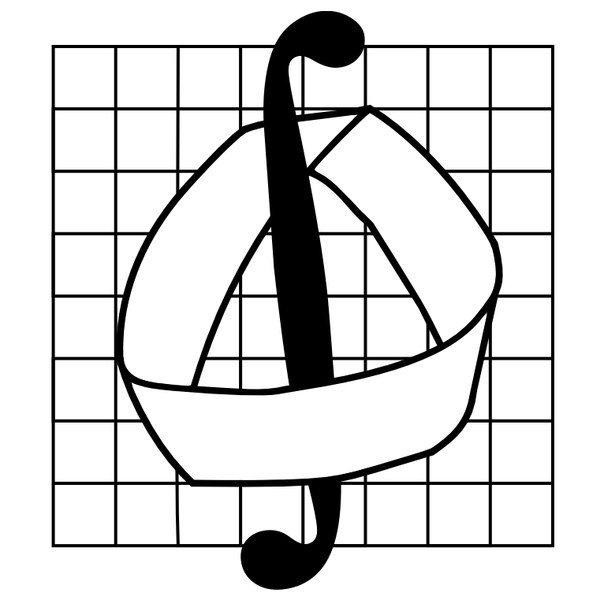
\includegraphics[width=6cm]{mmlogo1}

\end{center}

\end{figure}


\begin{center}
{\LARGE \bf ПОСТРОЕНИЕ РЕКОМЕНДАТЕЛЬНОЙ СИСТЕМЫ, ОСНОВАННОЙ НА ИТЕРАЦИОННОМ УЛУЧШЕНИИ ТОЧНОСТИ КЛАССИФИКАЦИИ\\
%\medskip
}\\
%\bigskip
%\medskip
%01.01.02 — дифференциальные уравнения
\end{center}
\vfill


\bigskip
\begin{flushright}
Дипломная работа студента группы 511\\
 Ведерникова Артема Викторовича\\
Научный руководитель:\\ к.т.н., к.ф.-м.н., доцент \\Рыжов А.П.\\
Рецензент: \\к.ф.-м.н., м.н.с. \\
Шуткин Ю.С. 
\end{flushright}
\vfill \vfill \centerline{Москва 2014} \break
\end{titlepage}